\section{The Magic Gem}
\label{sec:gem}

Let $S=(s_{ij})$ be an arrangement of order $n$, with cells indexed by $i,j\in\{0,\dots,n-1\}$ ($i$ the row from the top, $j$ the column from the left), and write $N=n^2$.

\begin{definition}[Gem coordinates]
\label{def:gem_coords}
To the cell $(i,j)$ assign the point $\mathbf p_{ij}=(x_{ij},y_{ij},z_{ij})\in\R^3$ with
\begin{equation}
x_{ij}=j-\frac{n-1}{2},\qquad y_{ij}=\frac{n-1}{2}-i,\qquad z_{ij}=s_{ij}-\frac{N+1}{2}.
\label{eq:gem_coords}
\end{equation}
The \emph{Magic Gem} of $S$ is the convex hull $\mathcal G(S)=\operatorname{conv}\{\mathbf p_{ij}\}$.
\end{definition}

The horizontal coordinates centre the grid at the origin, with the $x$-axis along the columns and the $y$-axis along the rows (top row at positive $y$); the vertical coordinate centres the entries so that the mean entry $(N+1)/2$ sits at height zero.
All three coordinates then have mean zero over the $N$ cells (\Cref{lem:variances}), so the origin is the centroid of the point set.
Each $\mathbf p_{ij}$ may equally be read as a vector from the centroid, and with unit masses at the points the point set is a rigid body whose centre of mass is the origin; \Cref{rem:inertia} records its inertia tensor.
Throughout the paper, the function $z=(z_{ij})$ on the grid is called the \emph{height function} of $S$.

\begin{example}[Lo Shu]
\label{ex:loshu}
For the Lo Shu square $S=\begin{pmatrix}2&7&6\\9&5&1\\4&3&8\end{pmatrix}$, $n=3$ and the centre value is $5$, so the nine points are
\[
\begin{array}{lll}
\mathbf p_{00}=(-1,1,-3), & \mathbf p_{01}=(0,1,2), & \mathbf p_{02}=(1,1,1),\\
\mathbf p_{10}=(-1,0,4), & \mathbf p_{11}=(0,0,0), & \mathbf p_{12}=(1,0,-4),\\
\mathbf p_{20}=(-1,-1,-1), & \mathbf p_{21}=(0,-1,-2), & \mathbf p_{22}=(1,-1,3).
\end{array}
\]
The centre cell maps to the origin and is the only point not on the hull; the gem has $f$-vector $(8,16,10)$ and volume $18$ (\Cref{fig:construction}).
\end{example}

\begin{proposition}[$D_4$-invariance]
\label{prop:symmetry_invariance}
Let $g\in D_4$ act on the grid and let $gS$ be the arrangement with $(gS)_c=s_{g^{-1}c}$.
Then $\mathcal G(gS)=\hat g\,\mathcal G(S)$, where $\hat g(x,y,z)=(g(x,y),z)$ is the isometry of $\R^3$ that applies the orthogonal map $g$ of the $(x,y)$-plane and fixes $z$.
In particular $\mathcal G(gS)$ and $\mathcal G(S)$ are congruent, and the gem is an invariant of the $D_4$-orbit of $S$.
\end{proposition}

\begin{proof}
In the centred coordinates \eqref{eq:gem_coords}, each $g\in D_4$ acts on the cell positions $(x_{ij},y_{ij})$ as an orthogonal map of the plane (a rotation by a multiple of $90^\circ$ or a reflection in a coordinate axis or a diagonal), and $(x_{gc},y_{gc})=g(x_c,y_c)$.
The point of $gS$ over the cell $gc$ has height $(gS)_{gc}=s_c=z_c+\frac{N+1}2$, i.e.\ the same height as the point of $S$ over $c$.
Hence the point set of $gS$ is $\{(g(x_c,y_c),z_c)\}_c=\hat g\{\mathbf p_c\}_c$.
An affine bijection maps the convex hull of a set to the convex hull of the image, so $\mathcal G(gS)=\hat g\,\mathcal G(S)$; $\hat g$ is an isometry because $g$ is orthogonal.
\end{proof}

Since the eight images are congruent, every essentially different magic square has one gem up to congruence; \Cref{sec:gem-geometry-880} shows that for $n=4$ the converse also holds except for the complement map $S\mapsto17-S$, which reflects the gem in the plane $z=0$.

\begin{figure}[htbp]
    \centering
    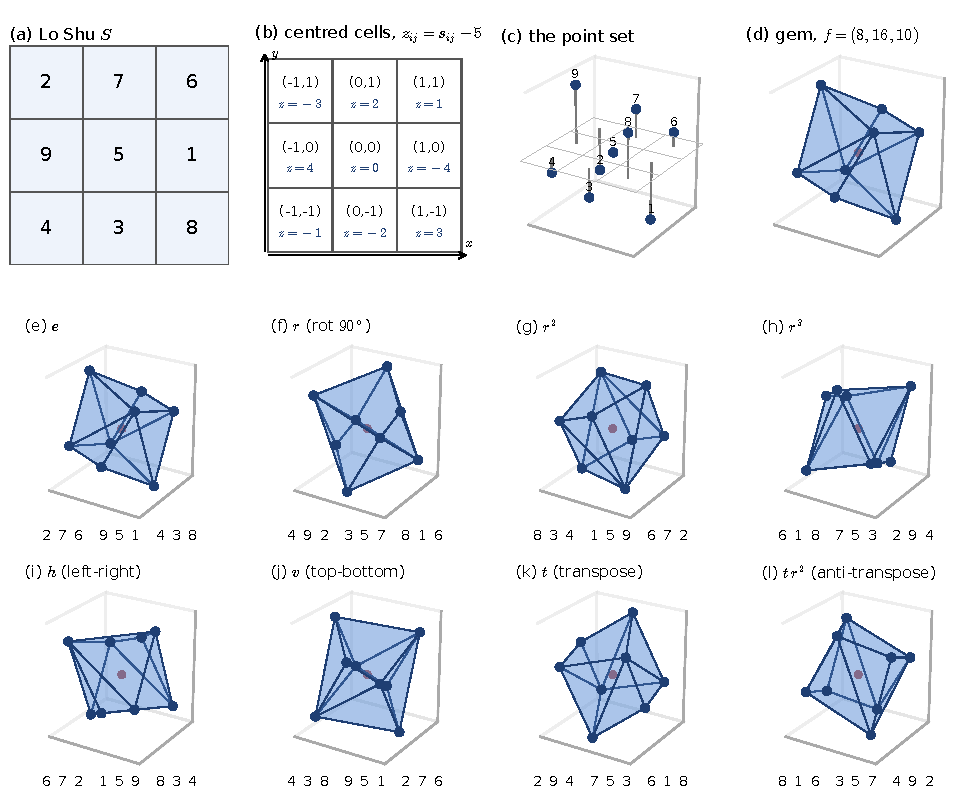
\includegraphics[width=\textwidth]{figures/fig01_construction_d4.pdf}
    \caption{Construction of the Magic Gem and its $D_4$-invariance.
    Top row: (a)~the Lo Shu square $S$; (b)~the centred cells $(x_{ij},y_{ij})$ with the heights $z_{ij}=s_{ij}-5$; (c)~the nine points $\mathbf p_{ij}$ over the grid, labelled by the entries $s_{ij}$; (d)~their convex hull, the gem of \Cref{ex:loshu}, with $f$-vector $(8,16,10)$; the centre point $(0,0,0)$ is the only interior point.
    Rows two and three (e--l): the eight images of the Lo Shu under $D_4$---the identity $e$, the rotations $r,r^2,r^3$ by $90^\circ,180^\circ,270^\circ$, the left--right and top--bottom reflections $h,v$, and the two diagonal reflections (transpose $t$ and anti-transpose $tr^2$)---each printed row by row beneath its gem.
    All eight gems are drawn from the same viewpoint; by \Cref{prop:symmetry_invariance} they are the images of one another under the isometries $\hat g$, so they are congruent, and all have $f$-vector $(8,16,10)$ and volume $18$.}
    \label{fig:construction}
\end{figure}
